\documentclass[a4paper,11pt]{article}
\pagestyle{headings}

\usepackage[utf8]{inputenc}
\usepackage{diagbox}
\usepackage[french]{babel}
\usepackage{graphicx}
\usepackage{float}
\usepackage{fullpage}
\usepackage{hyperref}
\usepackage{diagbox}
\usepackage{enumitem}
\usepackage[T1]{fontenc}
\usepackage[]{algorithm2e}
\usepackage{url}
\usepackage{array}
\usepackage{amsmath}
\graphicspath{{images/}}

\title{Reconnaissance de formes et apprentissage automatique Projet 3}
\author{Auriane Reverdell, Felix Hähnlein, Nicolas Violette, Romain Duléry}
\date{\today}

\setlength{\oddsidemargin}{0.2cm}
\setlength{\evensidemargin}{-0.7cm}
\setlength{\parindent}{30pt}
\setlength{\textwidth}{15cm}
\setlength{\textheight}{24cm}
\setlength{\topmargin}{-.3in}
\setlength{\parskip}{1ex}


\begin{document}

\maketitle
\vspace{1cm}

\section{Problématique et objectifs}

\section{Utilisation de notre propre réseau de neurones}

    Pour se rendre compte de l'éventail des difficultés liées au Deep Learning et afin de mieux comprendre son fonctionnement, il est important d'implémenter et d'entraîner son propre réseau de neurones.
    En effet, nous pouvons distinguer deux étapes bien différentes, la construction du réseau de neurones et son entraînement.

\subsection{Construction du réseau de neurones}
    
    Le choix du design d'un réseau de neurones est loin d'être une tâche triviale.
    Selon la problématique, la taille des données d'entrée et le temps que nous avons à notre disposition, l'architecture appropriée peut largement varier.
    Même pour un problème donné, les architectures ont beaucoup varié pendant les dernières décennies, grâce à l'amélioration du matérial utilisé et la programmabilité croissante du GPU.
    Effectivement, la complexité d'un réseau de neurones est directement liée au temps d'entraînement ce qui nous conduit à opter pour des réseaus plus profonds et des couches plus larges pendant ces dernières années.
    \\
    Alors qu'il est difficile de théoriser l'architecture à choisir, nous pouvons quand même faire quelques remarques par rapport à notre problème:
    \begin{itemize}
        \item
            Nous avons au moins besoin de 3 couches convolutionnelles si nous voulons détecter des feautures de bas niveau, moyen niveau et haut niveau.
            Ce comportement a été montré dans les travaux de Zeiler et al. \cite{zeiler2014visualizing}.
            Chacune de ces couches se construit par aggrégation de parties de la couche précédente.
        \item
            Après les couches convolutionnelles, nous retrouvons souvent au moins une couche complètement connectée avec un nombre de neurones important.
            Cette couche sert à mettre en relation les features de haut niveau. 
            Par exemple, un visage dispose de 2 yeux alignées.
            Tandis que la couche convolutionnelle de haut niveau va détecter la présence d'un oeil, la couche complètement connectée va pouvoir nous dire si nous en avons deux juste au-dessus du nez.
        \item
            En sortie de la toute dernière couche, nous retrouvons autant de neurones que de classes à distinguer.
            Ici, il est important à noter que le problème de détection peut être considéré comme un problème de détection appliqué à des sous-images.
            Par rapport à notre problème, cela veut dire que nous avons deux neurones de sortie, donnant la probabilité que l'imagette appartient à un visage ou pas.
    \end{itemize}

    Étant donné qu'il s'agit de notre première expérience construction de réseaux de neurones, nous nous sommes fortement inspirés d'un réseau d'un projet \textit{GitHub} \cite{face_detect} existant, accomplissant la même tâche avec approximativement la même taille de données d'entrée.
    \\
    L'architecture utilisée est resumée dans la table \ref{tab:network_architecture}. Le réseau prend en entrée des imagettes de taille $32\times32$.
    \\
    En plus des considérations précédentes, nous pouvons remarquer que chaque couche convolutionnelle est suivie d'une couche de sous-échantillonnage qui sert à réduire le nombre de paramètres filtrant les plus importants.
    \begin{table}
        \begin{tabular}{|l|c|c|c|c|c|c|c|r|}
            
            \hline
            \textbf{Layer} & Conv1 & MaxPool & Conv2 & MaxPool & Conv3 & MaxPool & Fc1 & Fc2 \\
            %colonne 1 & colonne 2 & colonne 3 & colonne 4 \\
            \hline
            \textbf{Kernel Size} & 5x5 & 2x2 & 3x3 & 2x2 & 3x3 & 2x2 & -  & - \\
            \textbf{Features} & 4 & - & 16 & - & 32 & - & 600  & 2 \\
            \hline
        \end{tabular}
        \caption{Architecture du réseau de neurones}
        \label{tab:network_architecture}
    \end{table}

\subsection{Paramètres d'entraînement}

    Pour nos premières expériences d'entraînement, nous avons utilisé des paramètres d'entraînement communément utilisé dans le cadre du framework \textit{Tensorflow}.
    \begin{itemize}
        \item{\textit{Fonction d'activation}} Softmax
        \item{\textit{Fonction de coût}} Entropie croisée
        \item{\textit{Taux d'apprentissage}} \verb$1e-4$
        \item{\textit{Taille des batchs}} $100$
    \end{itemize}

\subsection{Entraînement du réseau de neurones}
    
    Pendant l'entraînement du réseau, il est important de pouvoir le diagnostiquer.
    Pour cela, il est utile d'afficher la précision d'entraînement et la précision de test.
    Ce que nous entendons ici par précision, c'est en fait l'\textit{accuracy} qui est donnée par $\frac{TP+TN}{TP+FP+TN+FN}$.
    Il s'agit du ratio de bonnes classifications.
    %Alors que cette métrique n'est peut-être pas la métrique la plus représentative 
    Cette métrique a deux avantages. 
    Premièrement, elle tient compte du problème de classification que nous voulons résoudre.
    Deuxièmement, elle est facile à obtenir, car elle est calculée directement à la sortie du réseau de neurones pour le calcul de la fonction de coût.
    \\
    Quand nous proposons un modèle, nous sommes toujours confronté à la question de savoir si il comporte trop de paramètres ou si il n'y en a pas assez, compte tenu de la complexité du problème.
    On dit qu'on est confronté à un problème de \textit{sur-ajustement} ou de \textit{sous-ajustement}.
    L'affichage des deux précisions nous permet de savoir dans lesquels des deux cas on se trouve.
    Sur la figure \ref{fig:overfitting_1}, nous constatons que la précision de test diminue, alors que celle d'entraînement ne cesse d'augmenter.
    En plus, les oscillations de la courbe de précision de test indiquent que le modèle utilisé n'arrive pas à généraliser les informations d'entrée de manière fiable.
    Nous sommes alors confrontés à un problème de sur-ajustement.
    Pour résoudre ces problèmes, nous avons appliqué des méthodes de régularisation (voir la section \ref{sec:regularization}.

	\begin{figure}[H]
	    \centering
	    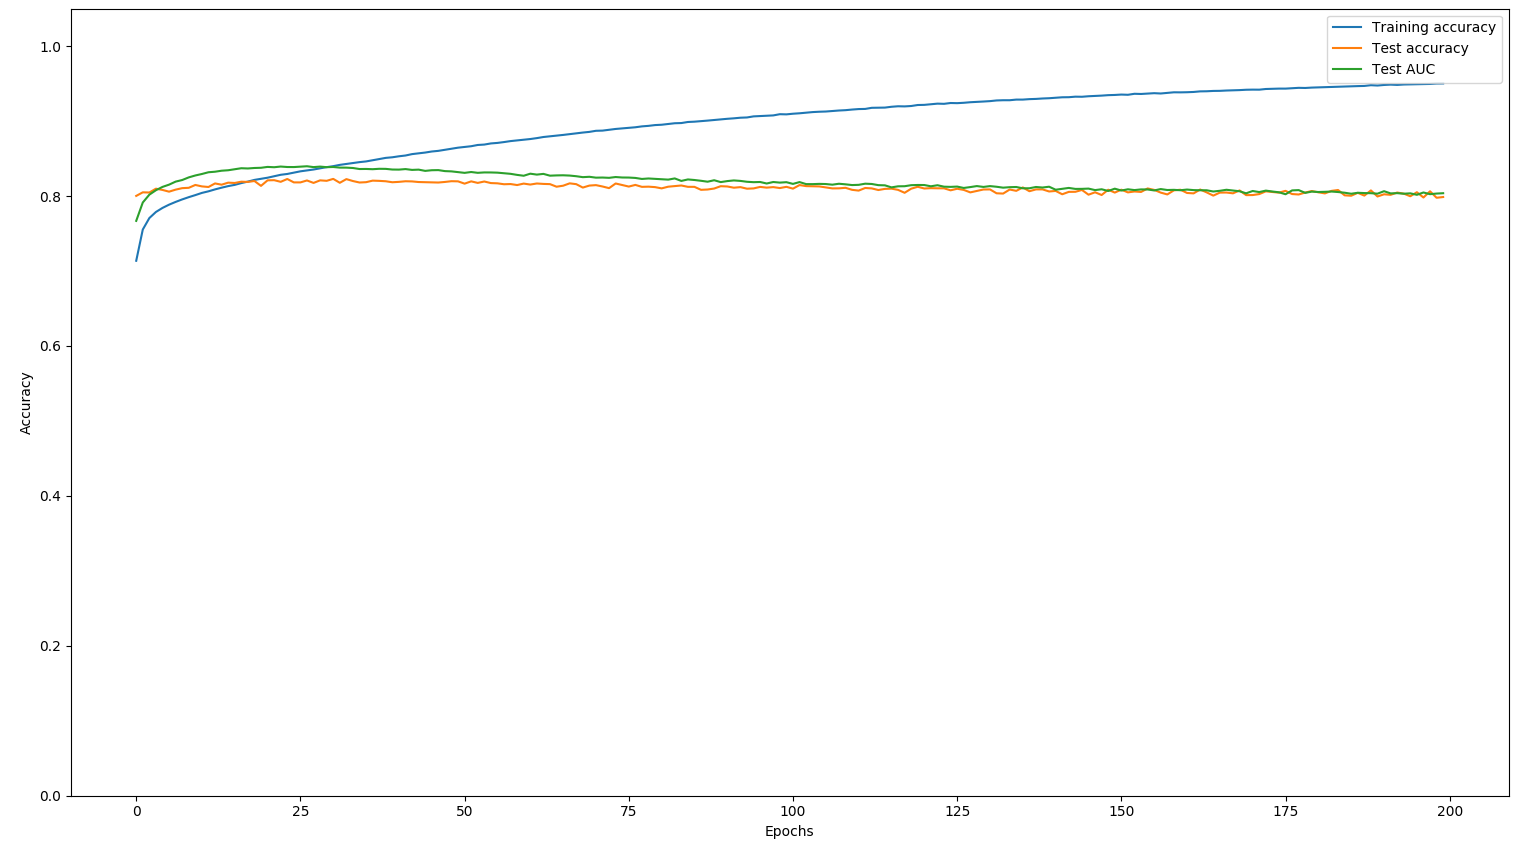
\includegraphics[scale=0.3]{overfitting_1.png}
	    \caption{Graphe des deux précisions. Nous sommes confrontés à un sur-ajustement du modèle.}
	    \label{fig:overfitting_1}
	\end{figure}

\subsection{Méthodes de régularisation}
\label{sec:regularization}
    
    Pendant la phase d'entraînement, nous avons besoin de pouvoir diagnostiquer le comportement du réseau.
    Pour mieux comprendre la régularisation d'un réseau de neurones, il est utile de se rappeler son fonctionnement.
    Un réseau de neurones est une méthode d'optimisation.
    Grâce à l'algorithme de \textit{rétropropagation du gradient}, il arrive à minimiser la fonction du coût en modifiant les poids et les bias.
    Autrement dit, l'algorithme cherche la meilleure solution dans l'espace des vecteurs de poids pour une fonction de coût donnée.
    Lors du sur-ajustement, quelques éléments de ce vecteur peuvent être disproportionnés par rapport au reste, il est alors biasé dans une certaine direction.
    L'algorithme d'optimisation va alors plus difficilement pouvoir explorer d'autres directions de l'espace de solutions.
    \\
    Les méthodes de régularisation visent à limiter la présence de ces poids abbérants.
    Nous avons testé les deux méthodes suivantes. 
    \begin{itemize}
        \item{\textit{Dropout}}

            La technique de dropout simule le disfonctionnement temporaire de nos neurones cérébrales.
            Elle s'applique à une ou plusieurs couches du réseau où elle enlève aléatoirement un certain nombre des neurones.
            Cela favorise la participation égale de toutes les neurones de la couche.
            Une illustration de cette méthode se trouve sur la figure \ref{fig:dropout_illustration}. 

        \item{\textit{La pénalisation des poids}}
            La méthode des pénalisations des poids consiste à rajouter un terme auxiliaire à la fonction de coût qui dépende de manière directe de la norme des poids du réseau.
            Voici un exemple de pénalisation de poids pour la norme $\mathcal{L}^2$.
            \begin{equation*}
                c = c_0 + \frac{\lambda}{n}\sum_{i=1}^n w_i^2
            \end{equation*}
        Remarquons que cette méthode va uniquement régulariser le réseau au sens de la norme utilisée.
    \end{itemize}

    Nous avons implémenté ces deux méthodes.
    Les résultats de la méthode de dropout se trouvent sur les figures \ref{fig:overfitting_with_dropout} et \ref{fig:overfitting_without_dropout}.
    Nous constatons que le sur-ajustement commence plus tard, environ à partir de l'époque 15 au lieu de l'époque 5, et que la précision de test a globalement augmenté.
    \\
    Sur la figure \ref{fig:l2_regularization}, nous avons visulaisé les résultats de l'entraînement en utilisant la deuxième méthode.
    Nous n'obtenons plus de sur-ajustement et des AUC (\textit{area under the curve}) de $0.891$ pour notre ensemble de test.
    À partir de l'époque 100, nous remarquons que les deux courbes sont plafonnées, alors qu'on obtient des performances comparables au premier projet qui utilisait des histogrammes RGB.
    Ce phénomène de saturation nous indique qu'on est maintenant confronté à un problème de sous-ajustement qui va être décrit dans la section \ref{sec:sous-ajustement}.

	\begin{figure}[H]
	    \centering
	    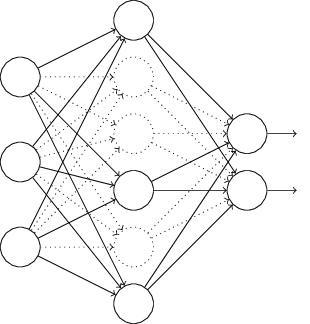
\includegraphics[scale=0.5]{dropout_illustration.png}
	    \caption{Illustration de la méthode de dropout. Les neurones en pointillés ne vont pas être "oubliés".}
	    \label{fig:dropout_illustration}
	\end{figure}

	\begin{figure}[H]
	    \centering
	    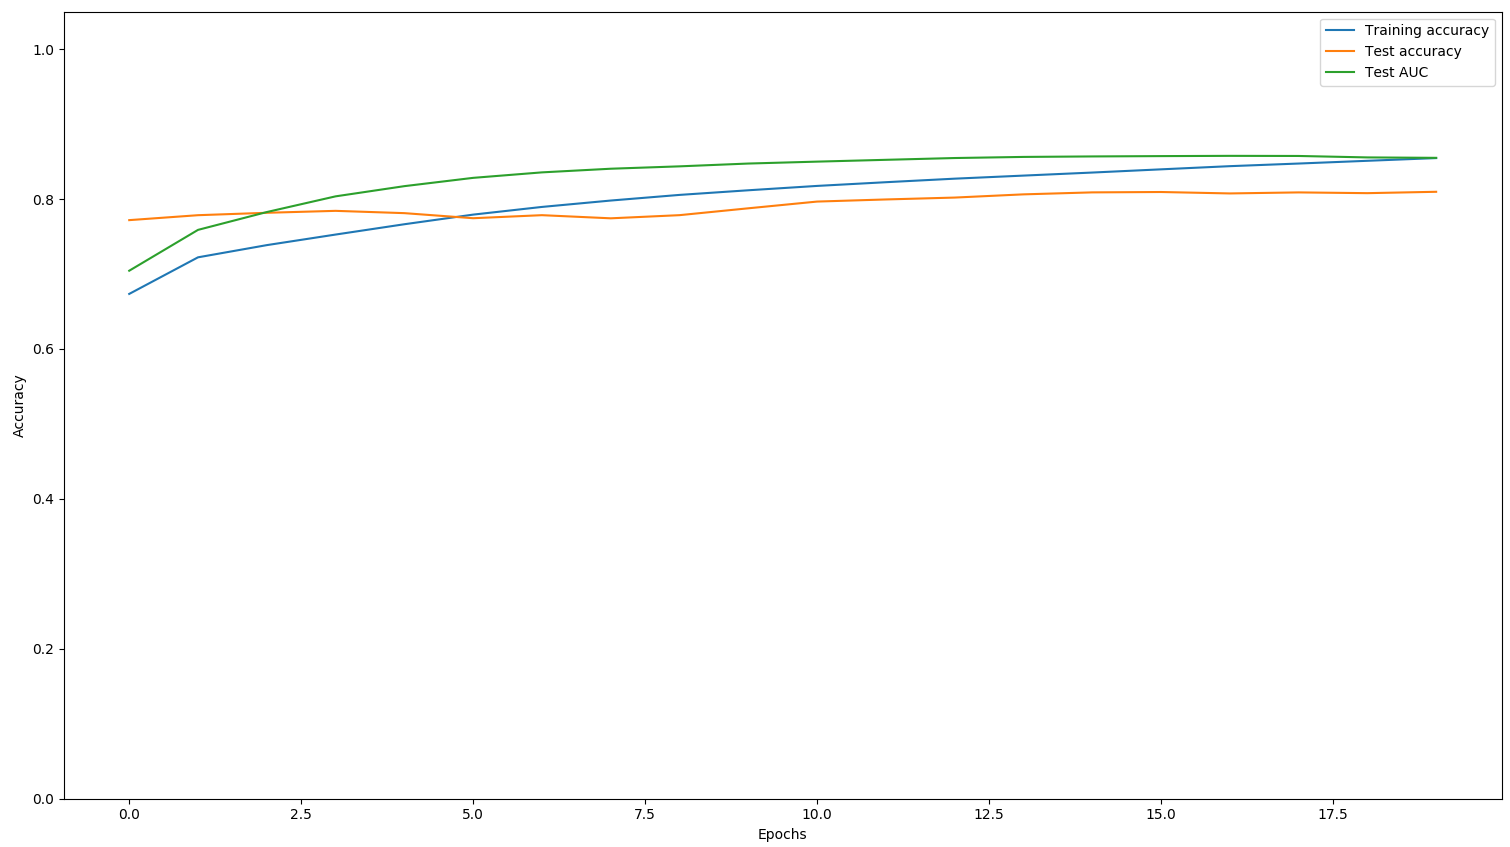
\includegraphics[scale=0.3]{overfitting_without_dropout.png}
	    \caption{Entraînement sans dropout}
	    \label{fig:overfitting_without_dropout}
	\end{figure}

	\begin{figure}[H]
	    \centering
	    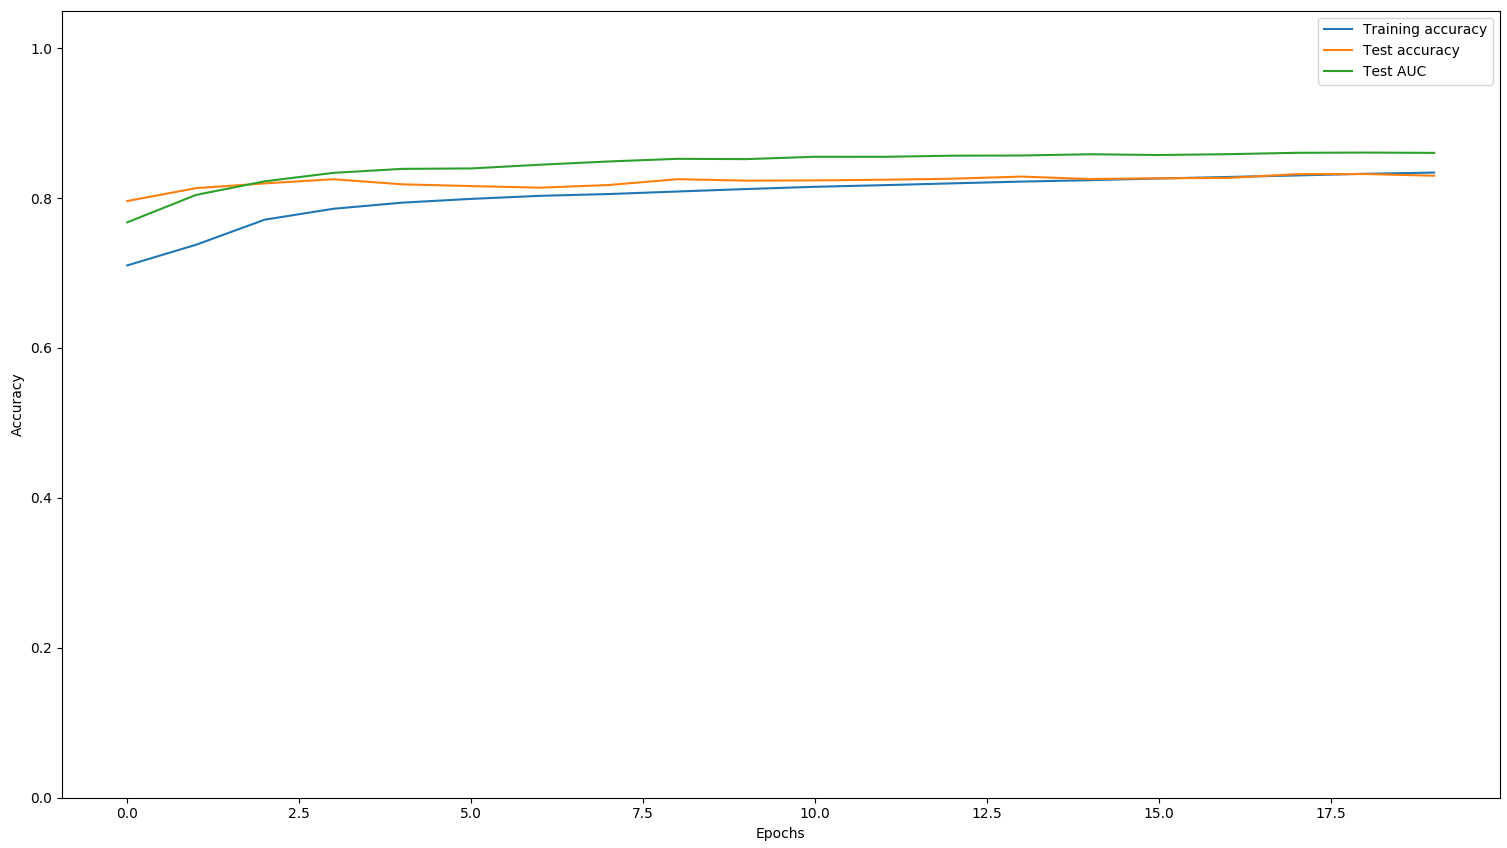
\includegraphics[scale=0.3]{overfitting_with_dropout.png}
	    \caption{Entraînement avec dropout}
	    \label{fig:overfitting_with_dropout}
	\end{figure}

	\begin{figure}[H]
	    \centering
	    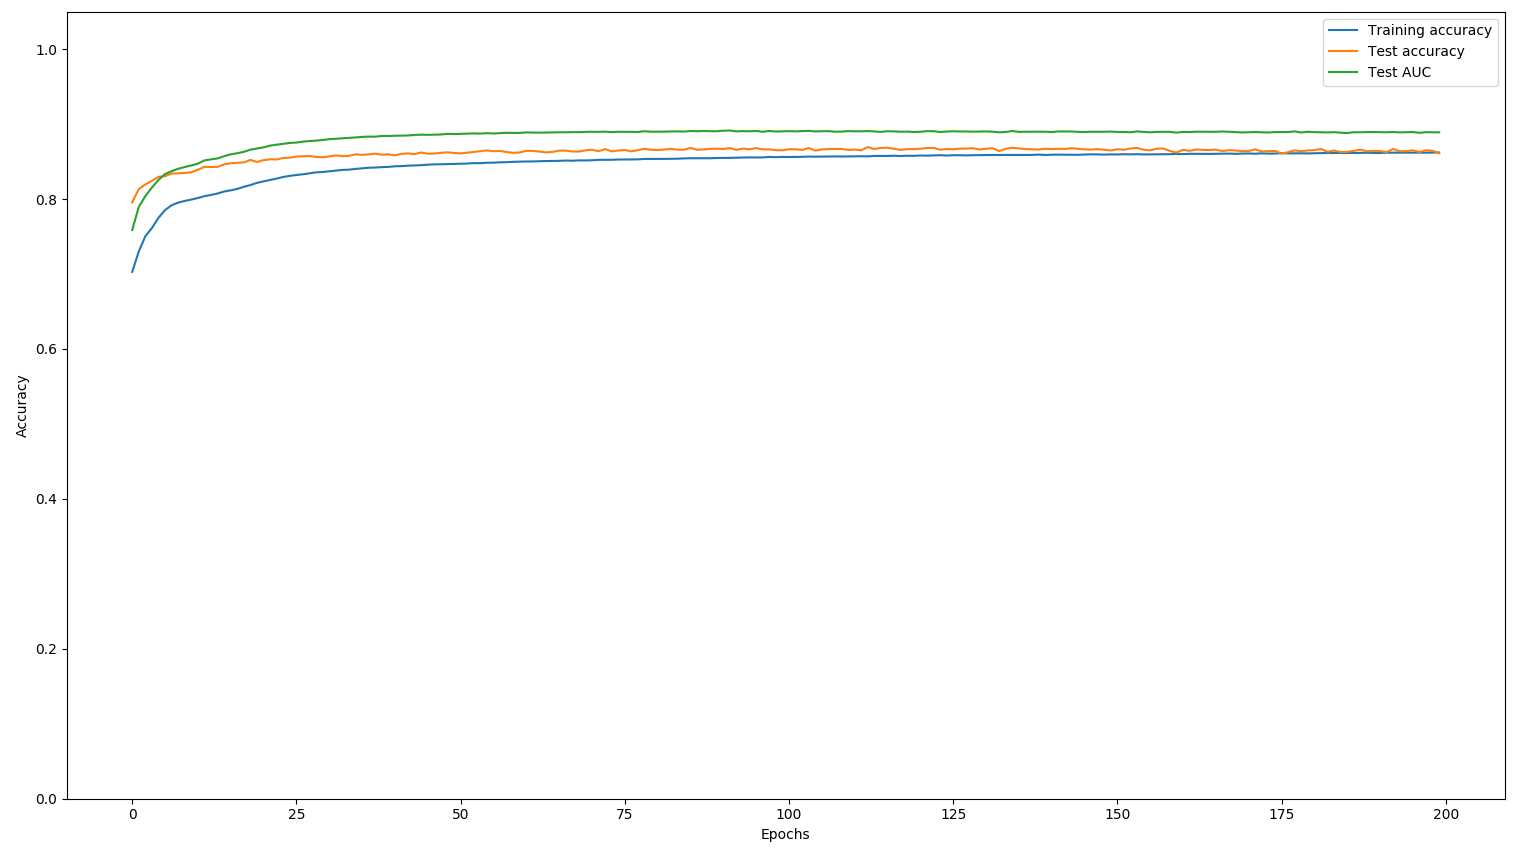
\includegraphics[scale=0.3]{l2_regularization_200.png}
	    \caption{Entraînement avec pénalisation de poids $\mathcal{L}^2$}
	    \label{fig:l2_regularization}
	\end{figure}

\subsection{Sous-ajustement}
\label{sec:sous-ajustement}

    Nous sommes face à un problème de sous-ajustement dans un des deux cas suivants.
    \begin{itemize}
        \item 
            Notre modèle n'est pas assez complèxe, i.e. ne comporte pas assez de paramètres, pour modéliser les données.
            Dans ce cas, il suffit d'augmenter la complexité du réseau de neurones, c'est-à-dire d'ajouter des couches ou d'augmenter le nombre de feautures par couche.
            Nous avons complexifié l'architecture de notre réseau, mais cela n'a pas augmenté sa performance.

        \item
            Les données utilisées pour l'entraînement ne sont pas asses représentatives pour modéliser le problème.
            Cela signifie dans notre cas, que des simples imagettes de taille $32\times32$ ne contiennent pas assez d'informations pour mener notre algorithme à la bonne décision.
            Nous avons pu vérifier cette hypothèse avec la méthode de \textit{transert learning} décrite dans la section \ref{sec:transfert_learning}.
            Nous avons entraîné un réseau avec deux tailles d'imagettes différentes.
            La précision finale est nettement meilleure avec des imagettes plus grandes en entrée. 
    \end{itemize}

    Nous nous sommes rendus compte que la détection basée sur des parties trop petites du visage pose des problèmes.
    Pour pallier le problème d'ajustement de la taille des imagettes, nous avons implémenté une pyramide d'images, comme l'a présenté un groupe pendant la séance de présentations.

\subsection{Pyramide d'images}

    L'idée de la pyramide d'images est de ne plus traiter l'image qu'à l'échelle originale, mais de traiter un ensemble d'images composé de l'image d'entrée à plusieurs échelles.
    L'avantage de cette structure par rapport à notre problème est que nous pouvons donner des visages entiers à notre réseau de neurones.
    Étant donné que l'imagette contient tout le visage, le réseau aura toutes les informations nécessaires pour prendre une décision.
    \\
    En pratique, nous extrayons tous les visages de la base de données \textit{WIDER} que nous redimensionnons.
    Ces images constituent notre ensemble d'images positives.
    Pour construire l'ensemble négatif, nous prenons un patch n'appartenant pas à une région de visage au hasard pour chaque visage extrait précédemment.
    À part des données d'entrées, nous n'avons rien changé par rapport à l'entraînement précédent.

\subsubsection{Détection de visages}
    
    Après avoir entrainé notre réseau, nous devons changer la manière que nous détectons des visages sur des nouvelles images.
    Pour cela, nous parcourons l'image à plusieurs échelles et nous redimensionnons les détections positives.
    Nous avons alors en sortie un ensemble de rectangles, que nous regroupons en utilisant la fonction \verb$groupRectangles$ de \textit{OpenCV}.

\subsubsection{Résultats}

    Nous avons entrainé le réseau en 200 époques et nous l'avons appliqué à des images provenant de la base de données \textit{FDDB}.
    Des exemples testés se trouvent sur les figures \ref{fig:first_scale} à \ref{last_scale}.

	\begin{figure}[H]
	    \centering
	    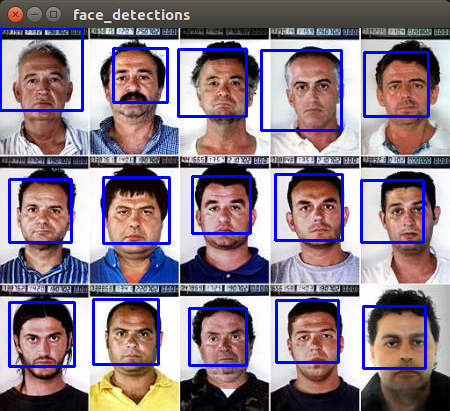
\includegraphics[scale=0.3]{first_scale.png}
	    \caption{Image évaluée avec la pyramide d'images}
	    \label{fig:first_scale}
	\end{figure}
	\begin{figure}[H]
	    \centering
	    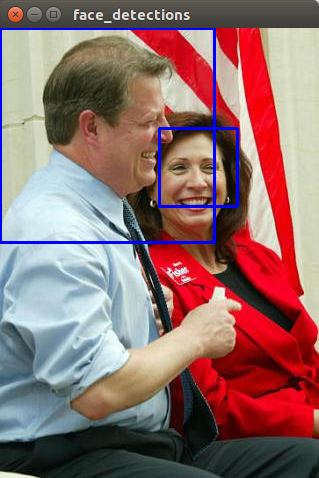
\includegraphics[scale=0.3]{scale_2.png}
	    \caption{Image évaluée avec la pyramide d'images}
	    \label{fig:scale_2}
	\end{figure}
	\begin{figure}[H]
	    \centering
	    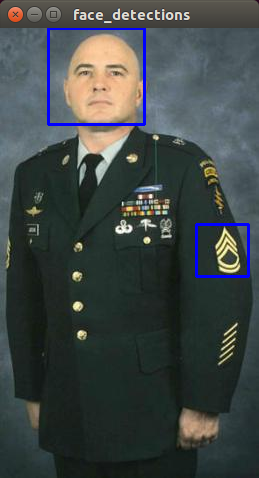
\includegraphics[scale=0.3]{scale_3.png}
	    \caption{Image évaluée avec la pyramide d'images}
	    \label{fig:scale_3}
	\end{figure}
	\begin{figure}[H]
	    \centering
	    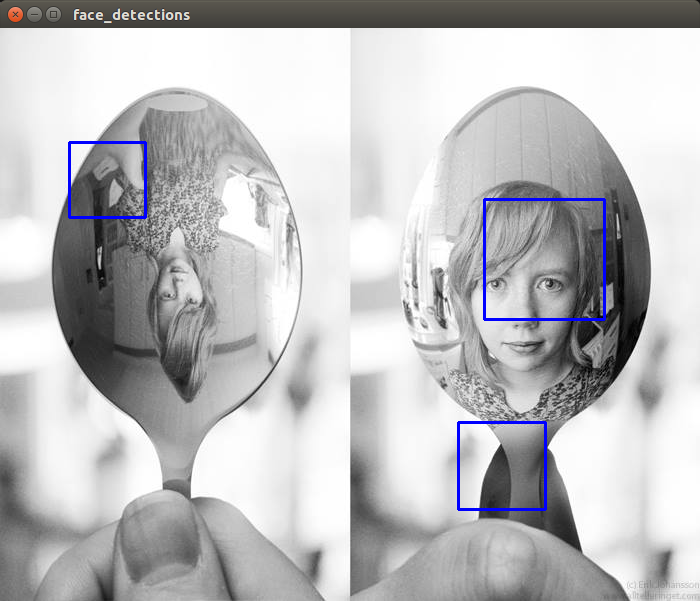
\includegraphics[scale=0.3]{last_scale.png}
	    \caption{Image évaluée avec la pyramide d'images}
	    \label{fig:last_scale}
	\end{figure}

    Nos tests nous montrent qu'on a obtenu une bonne amélioration grâce à l'utilisation de la pyramide d'images.
    En plus de cela, le regroupement des détections positives filtre davantage les faux positifs.
    Un exemple sans filtrage se trouve sur la figure \ref{fig:without_filter}.

	\begin{figure}[H]
	    \centering
	    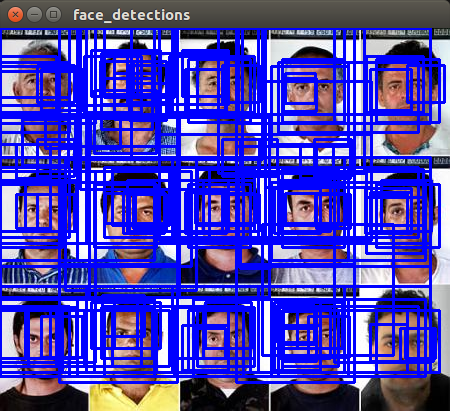
\includegraphics[scale=0.3]{without_filter.png}
	    \caption{Figure \ref{fig:first_scale} sans regroupement de rectangles}
	    \label{fig:without_filter}
	\end{figure}

\subsection{Evaluation des résultats}
\subsubsection{Evaluation par courbes ROC et Precision-Recall}
\subsubsection{Visualisation des filtres obtenus}

\section{Apprentissage par transfert : Réseaux de neurones pré-entraînés}
\subsection{Présentation de la méthode utilisée}
\label{sec:transfert_learning}

L'idée de l'apprentissage par transfert (\textit{fine-tuning}) est une spécialisation de
l'apprentissage dans un domaine particulier. Il s'agit de se fonder sur un réseau pré-entraîné sur
une grande base de données, et continuer de l'entraîner dans le domaine qui nous intéresse, ici la reconnaissance faciale.

Etant donné que les bases de données originales sont énormes, le modèle pré-entraîné aura déjà appris des features pertinents pour notre problème.

Par ailleurs, l'apprentissage par transfert est applicable à notre problème car il est généralisable
lorsque l'on enlève les couches supérieures.

Etant donné que notre base de données de test est relativement petite, l'apprentissage par transfert pourrait amener au surapprentissage (\textit{overfitting}), on utilise donc des stratégies de complétion des données d'entrée, comme présenté dans la partie \ref{sec:completion}.

    \subsection{Entraînement}
    \subsection{Evaluation des résultats}

\section{Utilisation d'un modèle plus complexe : Facenet}

    Facenet est un outil de reconnaissance faciale, fondé sur un MTCNN (multi-task CNN) pré-entraîné pour la détection de visage. Nous avons utilisé une implémentation Tensorflow de l'article \href{https://arxiv.org/abs/1503.03832}{FaceNet: A Unified Embedding for Face Recognition and Clustering}

    \subsection{Analyse qualitative des résultats}
	\subsubsection{True positives}

	    Facenet a réussi à faire face à des situations compliquées, comme par exemple la détection de visages flous, ou la non-détection de visages qui sont en réalité une projection sur un écran :\\
	    
	    \begin{figure}[H]
	        \centering
	        \begin{minipage}[c]{0.58\linewidth}
	            \begin{center}
	                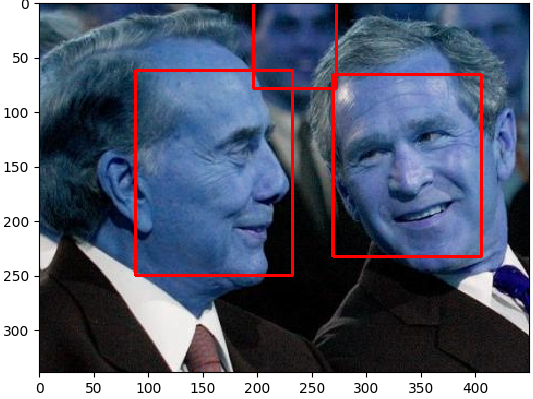
\includegraphics[scale=0.45]{facenetTP1.png}
	                \caption{Détection d'un visage flou en arrière plan}
	            \end{center}
	        \end{minipage} \hfill
	        \begin{minipage}[c]{0.35\linewidth}
	            \begin{center}
	                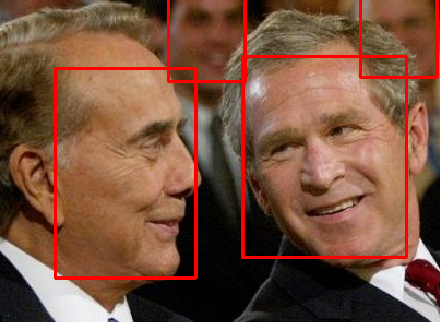
\includegraphics[scale=0.45]{facenetTP2.png}
	                \caption{Non détection d'un visage projeté sur un écran}
	                \label{fig:proj_ecran}
	            \end{center}
	        \end{minipage}
	    \end{figure}
	    
	    En réalité le visage projeté de la figure \ref{fig:proj_ecran} est considéré comme ground truth par FDDB mais cela peut être contestable étant donné la qualité de l'écran. De plus le visage projeté est détecté en utilisant des seuils plus permissifs.\\
	    
	\subsubsection{False positives}
	    
	    Par ailleurs, il y a des situations où la détection est erronée, mais pour lesquels on peut comprendre l'origine de l'erreur :\\
	    
	    \begin{figure}[H]
	        \centering
	        \begin{minipage}[c]{0.45\linewidth}
	            \begin{center}
	                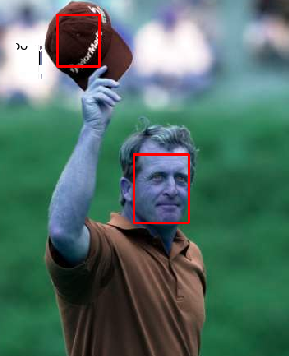
\includegraphics[scale=0.60]{facenetFP1.png}
	                \caption{Faux positif lié à l'apprentissage de la corrélation visage-casquette}
	            \end{center}
	        \end{minipage} \hfill
	        \begin{minipage}[c]{0.45\linewidth}
	            \begin{center}
	                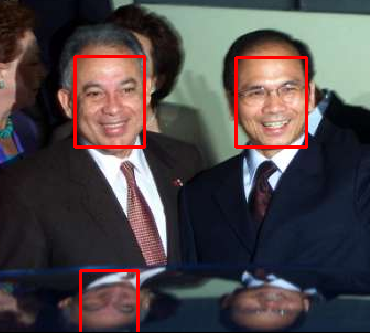
\includegraphics[scale=0.45]{facenetFP2.png}
	                \caption{Faux positif lié à la présence d'un visage en arrière-plan}
			\label{fig:fp}
	            \end{center}
	        \end{minipage}
	    \end{figure}

	    Dans la figure \ref{fig:fp}, la figure detectée derrière la main peut être considérée comme
	    juste (par un humain) du fait qu'un visage est bien présent derrière. Il est cependant consiéré comme
	    faux positif car il n'y a pas de vérité terrain à cet endroit là. Cela est peut-être du
	    au fait que la base de données FDDB n'est pas considérée comme étant une base de données
	    difficile.
	    
	    \begin{figure}[H]
	        \begin{center}
	            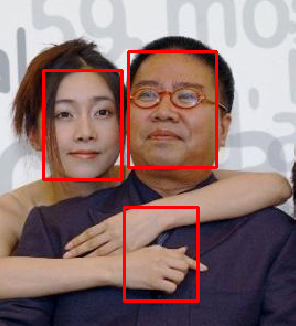
\includegraphics[scale=0.45]{facenetFP5.png}
	            \caption{Faux positif lié à l'apparence de la voiture en arrière-plan}
	        \end{center}
	    \end{figure}
	    
	    \newpage
	    Il y a également des faux positifs non explicables :\\
	    
	    \begin{figure}[H]
	        \centering
	        \begin{minipage}[c]{0.50\linewidth}
	            \begin{center}
	                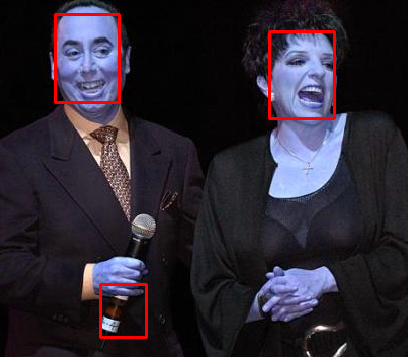
\includegraphics[scale=0.45]{facenetFP3.png}
	                \caption{Faux positif inexplicable}
	            \end{center}
	        \end{minipage} \hfill
	        \begin{minipage}[c]{0.45\linewidth}
	            \begin{center}
	                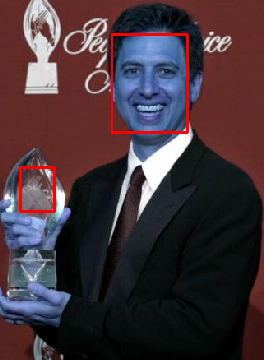
\includegraphics[scale=0.45]{facenetFP4.png}
	                \caption{Faux positif inexplicable}
	            \end{center}
	        \end{minipage}
	    \end{figure}
	    
	    \subsubsection{False negatives}
	    
	    La très grande majorité des faux négatifs sont dus à des situations compliquées, comme des soucis de luminosité, des visages tronqués, ou des visages flous en arrière-plan.\\
	    
	    \begin{figure}[H]
	        \centering
	        \begin{minipage}[c]{0.45\linewidth}
	            \begin{center}
	                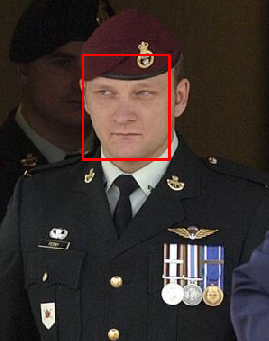
\includegraphics[scale=0.45]{facenetFN1.png}
	                \caption{Faux négatif du à la luminosité}
	            \end{center}
	        \end{minipage} \hfill
	        \begin{minipage}[c]{0.50\linewidth}
	            \begin{center}
	                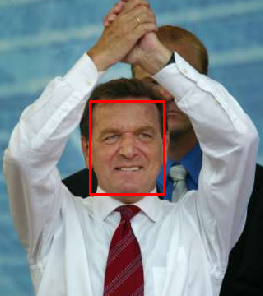
\includegraphics[scale=0.47]{facenetFN2.png}
	                \caption{Faux négatif du à la position du visage}
	            \end{center}
	        \end{minipage}
	    \end{figure}
	    
	    \begin{figure}[H]
	        \centering
	        \begin{minipage}[c]{0.50\linewidth}
	            \begin{center}
	                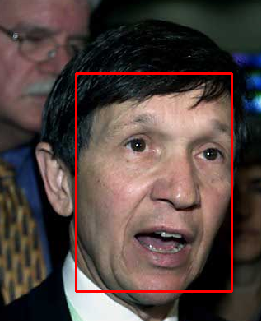
\includegraphics[scale=0.45]{facenetFN3.png}
	                \caption{Faux négatif du au flou}
	            \end{center}
	        \end{minipage} \hfill
	        \begin{minipage}[c]{0.45\linewidth}
	            \begin{center}
	                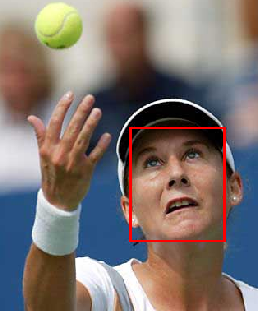
\includegraphics[scale=0.52]{facenetFN4.png}
	                \caption{Faux négatif du au flou}
	            \end{center}
	        \end{minipage}
	    \end{figure}

\section{Complétion de la base de données d'entrée}
\label{sec:completion}
    
    \subsection{Nécessité de compléter la base de données}

	La nécessité d'augmenter la base de données provient du fait que la performance des
	algorithmes de deep learning est directement proportionnelle à la taille de la base de
	données (figure \ref{fig:data1}). Il est donc intéressant d'augmenter les données déjà présentes
	lorsque nous n'avons pas de données supplémentaire à utiliser.

	\begin{figure}[H]
	    \centering
	    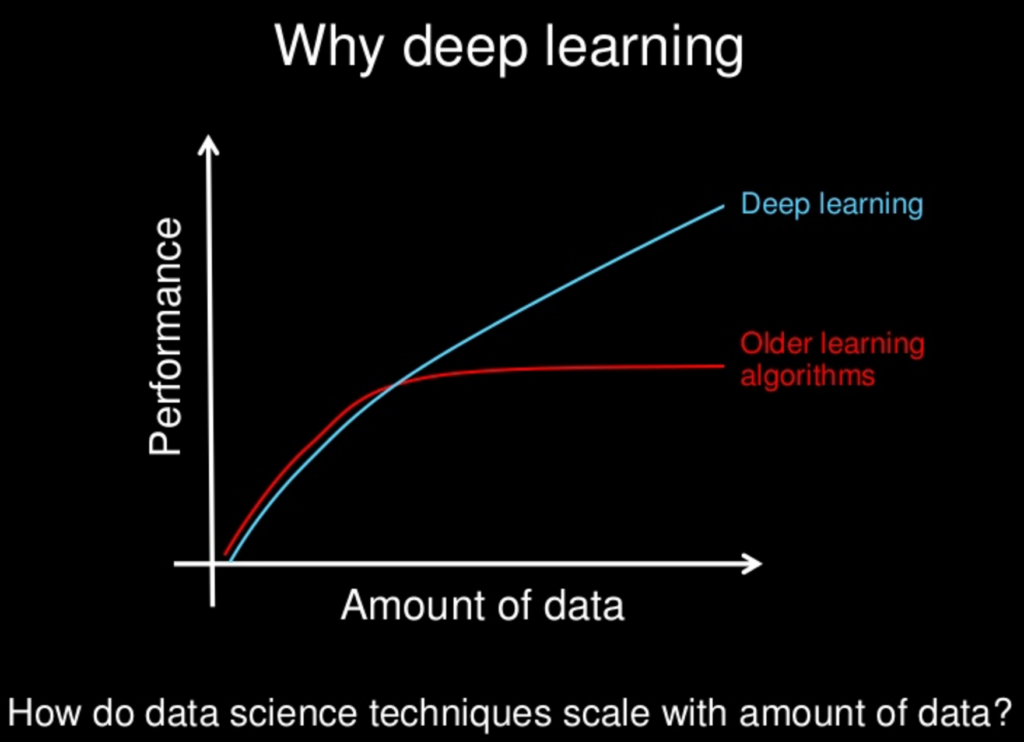
\includegraphics[scale=0.3]{deeplearning_data.png}
	    \caption{Graphe de performance en fonction du nombre de données}
	    \label{fig:data1}
	\end{figure}

    \subsection{Méthodes de complétion}

	Pour ce qui est des différentes méthodes d'augmentation, nous pouvons performer des
	transformations géométriques (translations, symétries, rotations) ou encore des
	déformations afin de reconnaître les photos prises avec des cameras "fisheyes".\\

	Il peut être intéressant d'altérer l'intensité de l'image de façon à reconnaître les images
	de test même si elles ont une amplitude d'intensité très variables. Nous pouvons par exemple
	citer la méthode de l'article AlexNet \cite{alexnet} qui prend l'intensité d'un pixel et lui
	rajoute un multiple des composantes principales de l'image (pour garder la valeur
	intrinsèque de l'image. Le multiple dépend des vecteurs propres de la matrice 3x3 de
	covariance du pixel et des valeurs propres de cette dernière multiplié par un coefficient
	de gaussienne de moyenne nulle et de variance $0.1$.\\

	Notre dernière idée consiste à appliquer un bruit blanc aux images afin de rendre
	l'algorithme moins sensible aux particularités d'une image mais plus au \textit{pattern}
	recherché.\\

	La représentation en RGB des images rajoute de la complexité (plus de dimensions) mais
	elle permet une meilleure performance du fait que la couleur humaine est particulière et se
	différencie grandement des couleurs d'arrière plan.

\newpage
\section{Annexes}
%http://ydwen.github.io/papers/WenECCV16.pdf
\bibliographystyle{unsrt}
\bibliography{sample}
%\flushleft [1] http://ydwen.github.io/papers/WenECCV16.pdf 
%[2] Zeiler, M. D., \& Fergus, R. (2014, September). Visualizing and understanding convolutional networks. In European conference on computer vision (pp. 818-833). Springer, Cham.

\end{document}
